\chapter{Algoritmos}
\label{sec:algoritmos}

Como se ha comentado previamente, se está trabajando sobre  un problema bastante peculiar, donde se intenta predecir distintas variables ordinales. Antes de comenzar con algoritmos más complejos, el primer enfoque para resolver el problema ha sido el de usar una media de cada variable a predecir. \\
Es cierto que usando este enfoque, estamos perdiendo información muy importante:  se está suponiendo que todas las variables son igualmente importantes, lo cual es una desventaja de esta aproximación al problema.
Por el contrario, este enfoque tiene la ventaja de estar usando algoritmos clásicos de regresión, proporcionando una salida más general, además de que usando este enfoque primero, descartamos la posibilidad de tener un conjunto de datos con mucho ruido o con un mal muestreo de los datos.\\
\linebreak
En esta sección vamos a explicar que algoritmos se han usado después del pre-procesamiento inicial.\\
Existe un teorema llamado\textbf{\textit{No-Free-Lunch}} que afirma no existe un algoritmo que resuelva los problemas de machine learning mejor que otro. Partiendo de esta idea, el objetivo principal de esta sección es el de comprobar el comportamiento de una serie de modelos e intentar mejorar el rendimiento de los mismos, añadiendo nuevos pasos a la etapa de pre-procesamiento y volviendo a entrenar los modelos que se han seleccionado. \\
\linebreak
\section{Conjuntos de validación}
\label{sec:validation}
Para ver el comportamiento de un modelo, no basta con definir un conjunto de entrenamiento para entrenar el modelo que se ha seleccionado y un conjunto de test para comprobar el comportamiento con datos que el algoritmo no conoce.  Aunque a primera vista esta parece una técnica correcta, tiene varios inconvenientes:
\begin{itemize}
	\item Cuando se ajustan los hiper-parámetros de los modelos,  se podría llegar a ajustar el modelo al conjunto de test, produciendo un sobre-ajuste.
	\item Solo se esta usando una parte de los datos para validar el modelo, nada asegura que el conjunto de test sea representativo del conjunto de datos con el que se está trabajando.
\end{itemize}
Para solventar estas y algunos otros problemas que que tiene esta metodología, se usa la \textbf{validación cruzada}.\\
\linebreak
En lugar de usar el conjunto de entrenamiento para entrenar un único modelo, se divide el conjunto de entrenamiento en $k$ partes, entrenando $k$ modelos usando $k-1$ subconjunto y usando el restante como de test. \\
\begin{figure}[H]
	\centering
	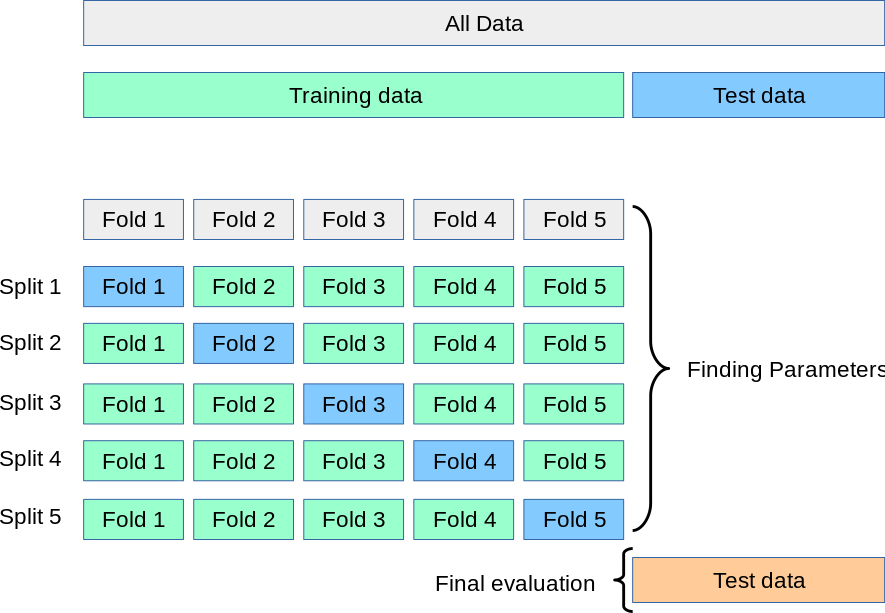
\includegraphics[scale=0.4]{grid_search_cross_validation.png}
	\caption{Ejemplo de validación cruzada con $k=5$}
	\label{fig:cross-validation}
\end{figure}
Como se aprecia en la figura \ref{fig:cross-validation},  se ha dividido el conjunto de datos en 5 conjuntos (folds), usando en cada iteración 4 para entrenar el modelo y uno para verificar con datos que el modelo no ha visto. Finalmente, se usa el conjunto de test (habiendo entrenado previamente el modelo con todo el conjunto de entrenamiento).